\section{Discussion}

% \begin{figure}[t]
% \centering
% \begin{subfigure}[b]{0.35\textwidth}
% \centering
% 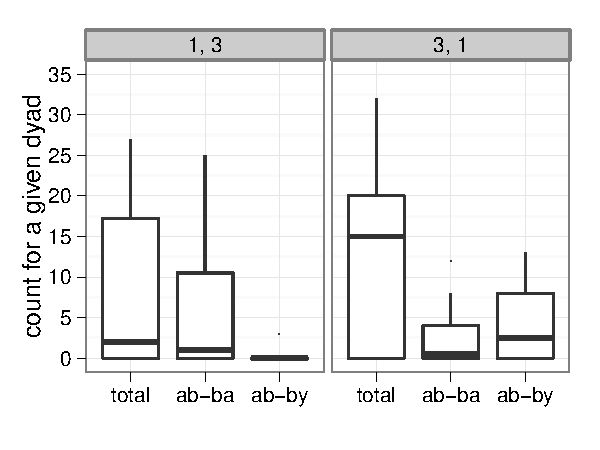
\includegraphics[scale=.5]{../figs/eckmann-small/example-obs-stats}
% %\caption{Observed counts}
% \end{subfigure}
% \qquad
% \begin{subfigure}[b]{0.35\textwidth}
% \centering
% 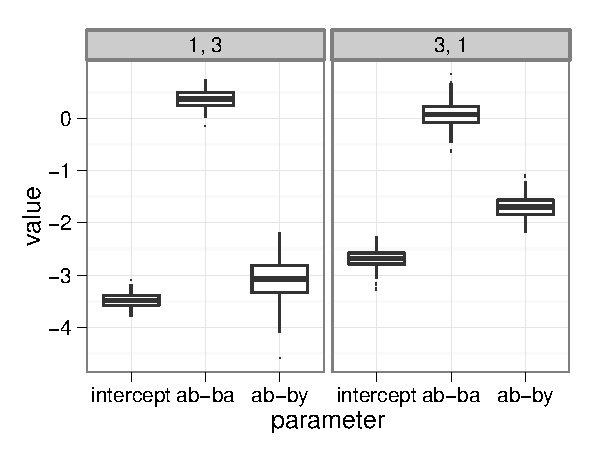
\includegraphics[scale=.5]{../figs/eckmann-small/example-estimates}
% %\caption{Samples of $\beta_{p,k,l}$}
% \end{subfigure}

% \caption{%Observed counts versus model estimates from Eckmann email data.
%  Left: Observed statistics across all dyadic email interactions between  members of group 1 and group 3.  Right: Posterior samples of the corresponding $\beta_{p,1,3}$ and $\beta_{p,3,1}$.  In addition to finding differences in mean activity for these dyads, estimates suggest events from 3 to 1 have a higher propensity for \texttt{ab-by} transitions.}
% \label{fig:posteriorparams}
% \end{figure}

\begin{figure}[t]
\centering
\begin{subfigure}[b]{0.22\textwidth}
\centering
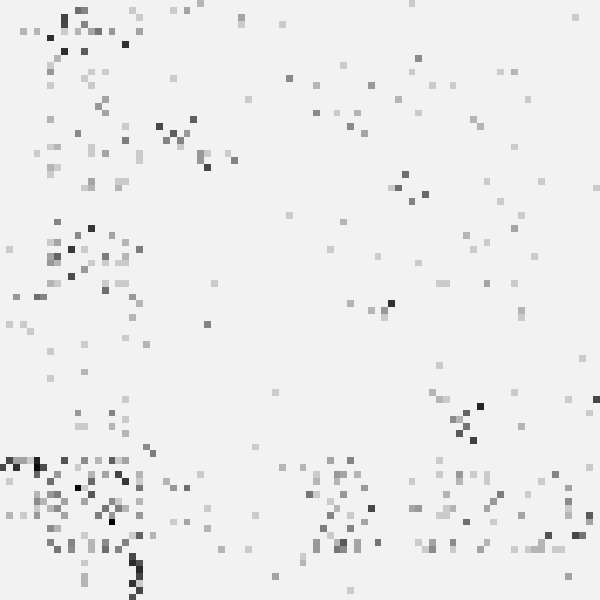
\includegraphics[scale=.25]{../figs/eckmann-small/parmat/observed}
\caption{Observed counts}
\end{subfigure}
~
\begin{subfigure}[b]{0.22\textwidth}
\centering
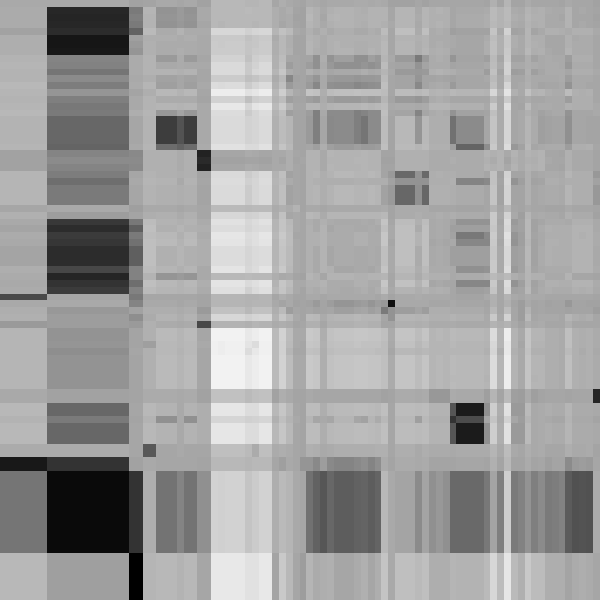
\includegraphics[scale=.25]{../figs/eckmann-small/parmat/1}
\caption{Intercept estimates}
\end{subfigure}
~
\begin{subfigure}[b]{0.22\textwidth}
\centering
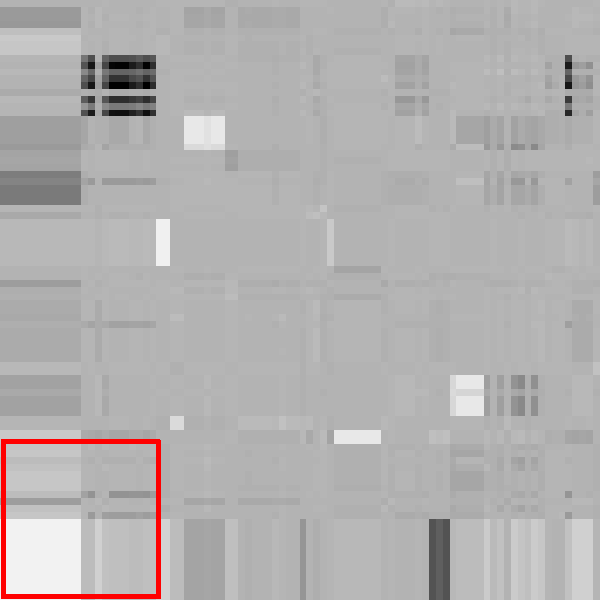
\includegraphics[scale=.25]{../figs/eckmann-small/parmat/2}
\caption{\texttt{ab-ba} estimates}
\end{subfigure}
~
\begin{subfigure}[b]{0.22\textwidth}
\centering
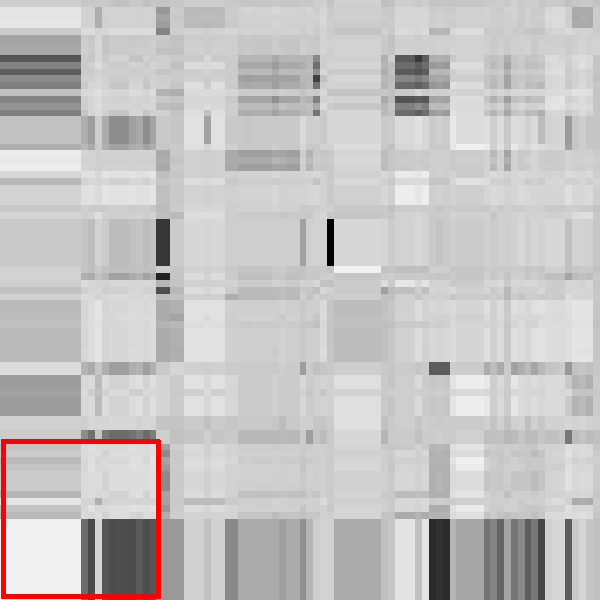
\includegraphics[scale=.25]{../figs/eckmann-small/parmat/3}
\caption{\texttt{ab-by} estimates}
\end{subfigure}
\caption{Comparing observed counts and parameter estimates.  Darker values are larger.  Estimates are rescaled posterior means $(\hat{\beta}_{p,z_i,z_j} - \hat{\mu}_p)/\hat{\sigma}_p$ for each dyad $(i,j)$.  Learned parameters suggest heterogeneity exists in both total activity (b) as well as dynamics, as seen in (c) and (d).}
\label{fig:parmats}
\end{figure}

 We propose a hierarchical approach for modeling event-based network data as a continuous-time Markov process.
Given a specification for the, the proposed method employs latent variables to model the heterogeneity in the event dynamics.
%is analogous to recent hierarchical extensions for latent position models \cite{Handcock2007} and exponential random graph models \cite{Schweinberger2011}.
%The method combines a latent variable framework (stochastic blockmodels) with a local dependence model for event sequences (relational event models \cite{Butts2008}).
%This provides detailed models of event dynamics among subsets of nodes while allowing for heterogeneity in the dynamics of the network as a whole.

This analysis suggests key differences exist in typical behaviors or roles that subsets of nodes share across a variety of data sets.
In Section \ref{sec:experiments} we show the model has improved predictive accuracy over baseline methods on real data with respect to ranking tasks and the likelihood of unobserved data.
We also note that we can improve over relational event models that lack latent clusters as well as stochastic blockmodels for count data, both special cases 
Other theories could be explored by including relevant statistics in the specification of $\mathbf{s}(t,i,j,\mathcal{A}_t)$, and similarly one can use our method to study how the roles of these statistics vary across nodes.

Relational event models \cite{Butts2008} require a knot at each observed event, while other approaches such as \cite{Gunawardana2011} learn the regions where an intensity is constant.
By using decision trees,  \cite{Gunawardana2011} also allow for a nonlinear relationship between statistics and intensity functions, while here we use latent variables to allow for heterogeneity in intensities across possible events.

Trivially extended to co-clustering applications and for directed data.
Also useful for our model when nodes belong to one latent class as a sender but another latent class as a recipient.

Our method learns about event dynamics within latent groups of individuals, but other types of heterogeneity likely exist in some data sets.
For example, dynamics might change over time \cite{Vu2011}.
Alternatively, if nodes change groups.
One approach, analogous to \cite{Airoldi2008}, would allow the latent class $z_i$ to be drawn from node-specific membership vectors $\pi_i$  after each change point.
In some contexts such extensions might be substantively important and warrant future work.
